\chapter{Project Management}
\section{Agile Development Methodology}
Teams use the agile development methodology to minimize risk (such as bugs, cost overruns, and changing requirements) when adding new functionality. In all agile methods, teams develop the software in iterations that contain mini-increments of the new functionality. There are many different forms of the agile development method, including scrum, crystal, extreme programming (XP), and feature-driven development (FDD).

\begin{figure}[H]
    \centering
    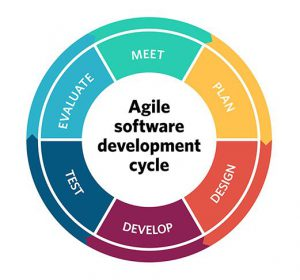
\includegraphics[scale = 0.9]{project_management/agile.jpg}
    \caption{Agile Development Methodology}
    \label{fig:Agile Development Methodology}
\end{figure}

\section{Trello}
Trello is a web-based project management and collaboration tool that allows users to organize tasks and projects using boards, lists, and cards. 

We have used trello's agile board template for project management and collaboration.
\begin{figure}[H]
    \centering
    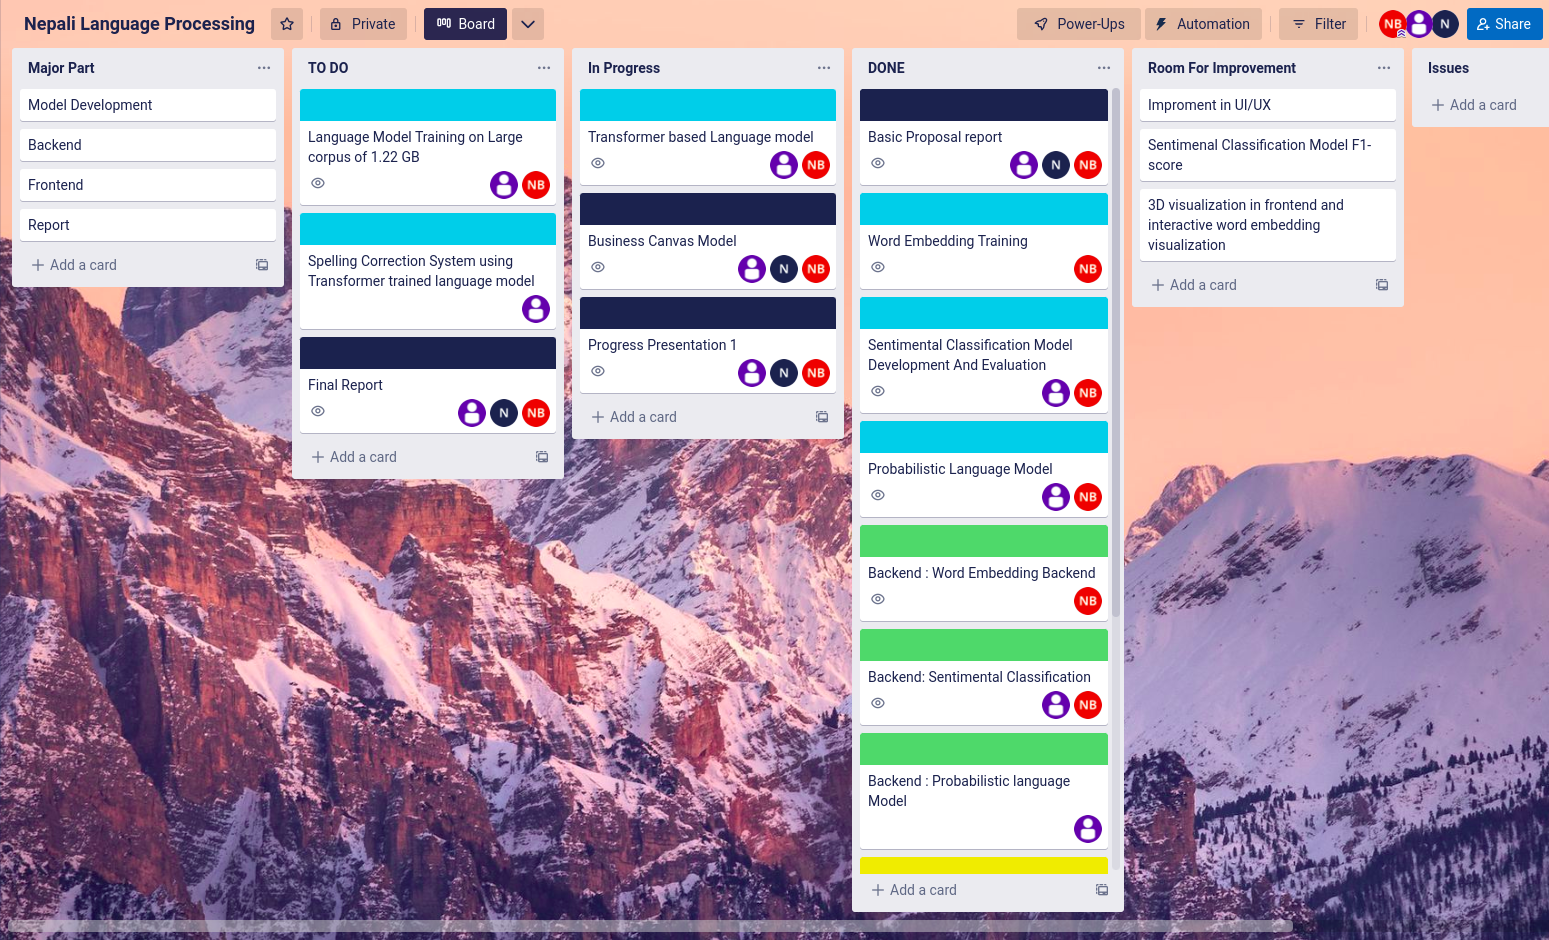
\includegraphics[scale = 0.25]{project_management/trello.png}
    \caption{Trello}
    \label{fig:Trello}
\end{figure}

\section{Discord}
We have used discord for effective communication and team meetings.

\begin{figure}[H]
    \centering
    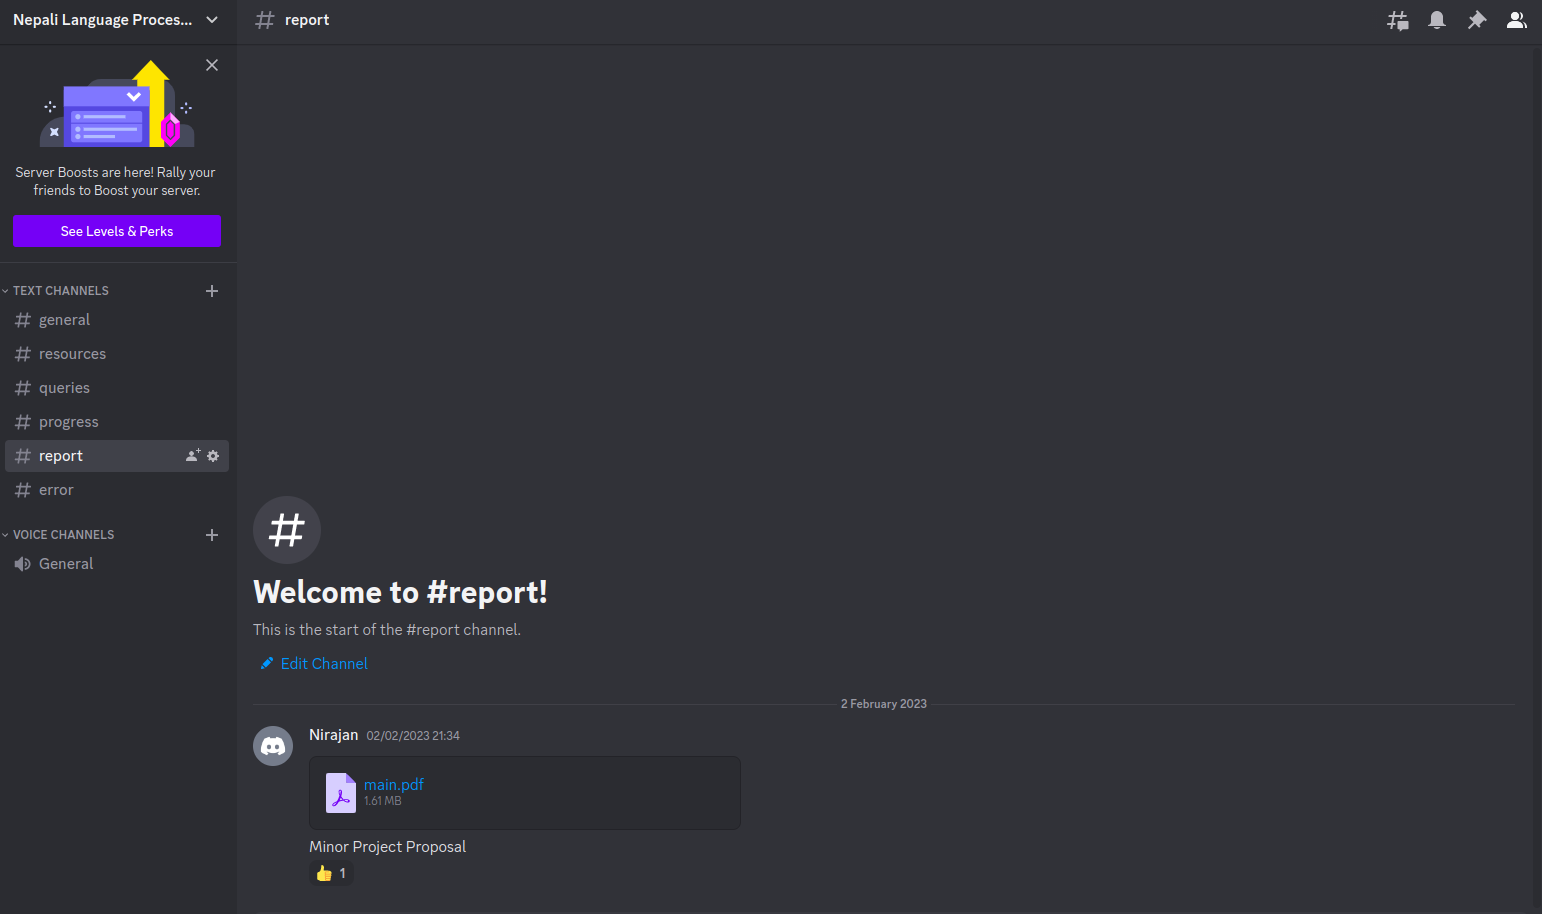
\includegraphics[scale = 0.25]{project_management/discord.png}
    \caption{Discord}
    \label{fig:Discord}
\end{figure}



